% diagrams/english/entrada.tex -- la entrada de casa de Lucía, para
% "Where is it?": la puerta con su felpudo, tres perchas en la pared y un
% banco con sitio debajo.
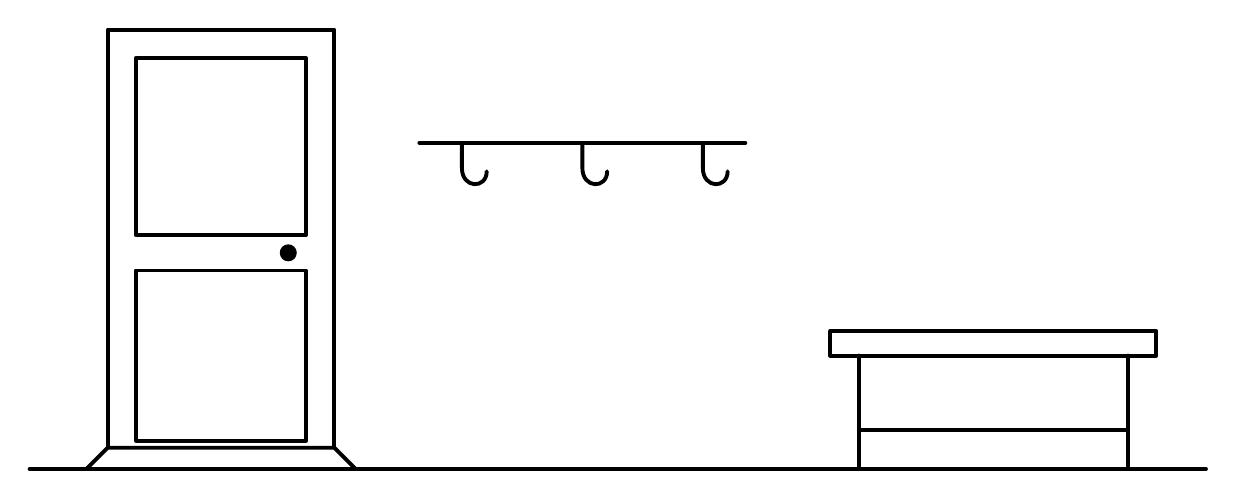
\begin{tikzpicture}[line width=1.4pt, line cap=round, line join=round, scale=0.9]
  \draw (-0.3,0) -- (16.3,0);
  % la puerta y el felpudo
  \filldraw[fill=white] (0.8,0) rectangle (4.0,6.2);
  \draw (1.2,0.4) rectangle (3.6,2.8); \draw (1.2,3.3) rectangle (3.6,5.8);
  \fill (3.35,3.05) circle (0.12);
  \filldraw[fill=white] (0.5,0) -- (0.8,0.3) -- (4.0,0.3) -- (4.3,0) -- cycle;
  % las perchas
  \draw (5.2,4.6) -- (9.8,4.6);
  \foreach \x in {5.8,7.5,9.2} {
    \draw (\x,4.6) -- (\x,4.25) .. controls (\x,3.95) and (\x+0.35,3.95) .. (\x+0.35,4.2);
  }
  % el banco
  \filldraw[fill=white] (11.0,1.6) rectangle (15.6,1.95);
  \draw (11.4,1.6) -- (11.4,0); \draw (15.2,1.6) -- (15.2,0);
  \draw (11.4,0.55) -- (15.2,0.55);
\end{tikzpicture}
